% =========================================================================
% Teaser (Figure 1) -- TikZ, built with OpenTikZ
%   Panel 1: standard competence readouts fail on duplex models
%   Panel 2: a mid-network (L22) linear read, before the first output token
%   Panel 3: live handoff -- the same talker speaks the expert answer
%
% Aspect is deliberately ~2.2:1 (not a thin strip): at \linewidth the whole
% picture only scales to ~0.70, which keeps the smallest label above 5.5pt.
% Build: tectonic -X compile teaser_tikz.tex
% =========================================================================
\documentclass[border=8pt]{standalone}

\usepackage[T1]{fontenc}
\usepackage{lmodern}
\usepackage{tikz}
\usepackage{amsmath}
\usetikzlibrary{positioning, arrows.meta, decorations.pathreplacing, calc}

% --- OpenTikZ palette (light / default, color-blind-friendly Okabe-Ito) ---
\definecolor{otblue}{HTML}{0072B2}
\definecolor{otorange}{HTML}{E69F00}
\definecolor{otteal}{HTML}{009E73}
\definecolor{otpurple}{HTML}{CC79A7}
\definecolor{otgray}{HTML}{5A5A5A}

% ---- reusable glyphs (adapted from OpenTikZ icons) ----------------------
% cloud silhouette (icons/systems/cloud), anchored near (#1,#2), scale #3, colour #4
\newcommand{\otcloud}[4]{%
  \begin{scope}[shift={(#1,#2)}, scale=#3]
    \begin{scope}
      \clip (-1.55,-0.45) rectangle (1.9,1.35);
      \fill[#4, rounded corners=0.4cm] (-1.25,-0.45) rectangle (1.7,0.35);
      \fill[#4] (-0.8,0.02) circle[radius=0.5];
      \fill[#4] (-0.1,0.42) circle[radius=0.55];
      \fill[#4] (0.65,0.18) circle[radius=0.72];
      \fill[#4] (1.25,-0.04) circle[radius=0.46];
    \end{scope}
  \end{scope}}

% lightning bolt = the gate decision; centred at (#1,#2), scale #3
\newcommand{\otbolt}[3]{%
  \begin{scope}[shift={(#1,#2)}, scale=#3]
    \filldraw[draw=otorange!75!black, fill=otorange, line join=round, line width=0.5pt]
      (0.14,0.52) -- (-0.30,0.02) -- (-0.02,0.02) -- (-0.14,-0.52)
      -- (0.30,-0.02) -- (0.02,-0.02) -- cycle;
  \end{scope}}

% failure cross at (#1,#2), arm #3
\newcommand{\otcross}[3]{%
  \draw[otpurple!75!black, line width=1.6pt, line cap=round]
    ($(#1,#2)+(-#3,-#3)$) -- ($(#1,#2)+(#3,#3)$)
    ($(#1,#2)+(-#3,#3)$) -- ($(#1,#2)+(#3,-#3)$);}

% success check at (#1,#2), arm #3
\newcommand{\otcheck}[3]{%
  \draw[otteal!75!black, line width=1.7pt, line cap=round, line join=round]
    ($(#1,#2)+(-#3,0.10)$) -- ($(#1,#2)+(-0.25*#3,-0.62*#3)$)
    -- ($(#1,#2)+(#3,0.78*#3)$);}

% speech arcs opening right, at (#1,#2), scale #3, colour #4
\newcommand{\otwaves}[4]{%
  \begin{scope}[shift={(#1,#2)}, scale=#3]
    \foreach \r in {0.26,0.48,0.70}{
      \draw[#4, line width=1.2pt, line cap=round]
        (0,0) ++(-42:\r) arc[start angle=-42, end angle=42, radius=\r];}
  \end{scope}}

% loudspeaker at (#1,#2), scale #3, colour #4
\newcommand{\otspeaker}[4]{%
  \begin{scope}[shift={(#1,#2)}, scale=#3]
    \filldraw[draw=#4!75!black, fill=#4!15, line width=1.1pt, line join=round]
      (-0.46,-0.20) -- (-0.16,-0.20) -- (0.20,-0.50) -- (0.20,0.50)
      -- (-0.16,0.20) -- (-0.46,0.20) -- cycle;
    \foreach \r in {0.24,0.44}{
      \draw[#4!75!black, line width=1.1pt, line cap=round]
        (0.28,0) ++(-45:\r) arc[start angle=-45, end angle=45, radius=\r];}
  \end{scope}}

\begin{document}
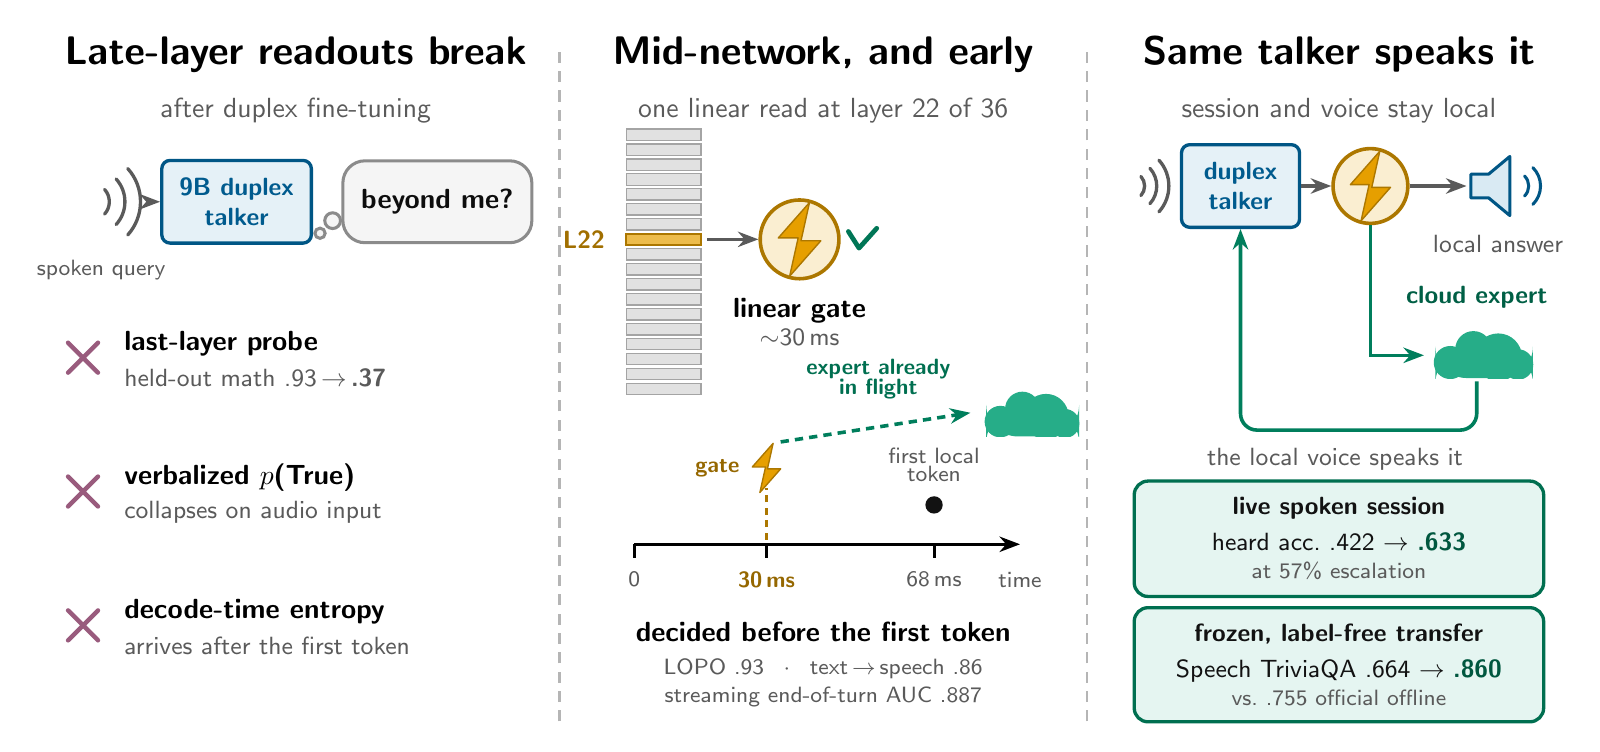
\begin{tikzpicture}[
    >={Stealth[length=2.6mm]},
    font=\sffamily,
    % ---- shared styles ---------------------------------------------------
    talker/.style={draw=otblue!75!black, fill=otblue!10, line width=1.2pt,
                   rounded corners=3pt, align=center,
                   font=\sffamily\bfseries\small, text=otblue!80!black,
                   inner sep=4pt},
    chip/.style={draw=otteal!70!black, fill=otteal!10, line width=1.2pt,
                 rounded corners=5pt, align=center,
                 font=\sffamily\small, text=otgray!20!black, inner sep=6pt},
    gatecirc/.style={draw=otorange!75!black, fill=otorange!18, line width=1.3pt,
                     circle, inner sep=0pt},
    lay/.style={draw=otgray!55, fill=otgray!18, line width=0.5pt},
    layhi/.style={draw=otorange!75!black, fill=otorange!70, line width=0.7pt},
    ptitle/.style={font=\sffamily\bfseries\Large, text=black, align=center},
    hd/.style={font=\sffamily\bfseries, text=black},
    sub/.style={font=\sffamily\small, text=otgray},
    ty/.style={font=\sffamily\footnotesize, text=otgray},
    flow/.style={->, draw=otgray, line width=1.2pt},
    esc/.style={->, draw=otteal!80!black, line width=1.3pt},
    escd/.style={->, draw=otteal!80!black, line width=1.3pt,
                 dash pattern=on 3pt off 2.2pt},
    divider/.style={draw=otgray!45, line width=1pt,
                    dash pattern=on 4pt off 3pt},
  ]

% =========================================================================
% PANEL 1 (x 0.0 .. 6.3) -- the standard readouts fail
% =========================================================================
\node[ptitle] at (3.15,8.55) {Late-layer readouts break\\[1pt]
  \normalsize\mdseries\color{otgray}after duplex fine-tuning};

% spoken query -> duplex talker -> "beyond me?"
\otwaves{0.55}{7.00}{0.90}{otgray}
\node[ty, anchor=north] at (0.68,6.38) {spoken query};

\node[talker] (t1) at (2.40,7.00) [minimum width=1.9cm, minimum height=1.05cm]
  {9B duplex\\talker};
\draw[flow] (1.28,7.00) -- (t1.west);

% thought bubble (tail = two shrinking circles, no arrow)
\draw[draw=otgray!70, fill=otgray!6, line width=1.1pt, rounded corners=8pt]
  (3.75,6.48) rectangle (6.15,7.52);
\node[font=\sffamily\bfseries, text=otgray!15!black] at (4.95,7.00) {beyond me?};
\draw[draw=otgray!70, fill=otgray!6, line width=1.1pt] (3.62,6.76) circle[radius=0.10];
\draw[draw=otgray!70, fill=otgray!6, line width=1.1pt] (3.46,6.60) circle[radius=0.065];

% three failed readouts
\otcross{0.45}{5.02}{0.19}
\node[hd, anchor=west]  at (0.85,5.20) {last-layer probe};
\node[sub, anchor=west] at (0.85,4.76) {held-out math .93\,$\to$\,\textbf{.37}};

\otcross{0.45}{3.32}{0.19}
\node[hd, anchor=west]  at (0.85,3.50) {verbalized $p$(True)};
\node[sub, anchor=west] at (0.85,3.06) {collapses on audio input};

\otcross{0.45}{1.62}{0.19}
\node[hd, anchor=west]  at (0.85,1.80) {decode-time entropy};
\node[sub, anchor=west] at (0.85,1.36) {arrives after the first token};

\draw[divider] (6.50,0.40) -- (6.50,9.00);

% =========================================================================
% PANEL 2 (x 6.7 .. 13.0) -- the mid-network read, before the first token
% =========================================================================
\node[ptitle] at (9.85,8.55) {Mid-network, and early\\[1pt]
  \normalsize\mdseries\color{otgray}one linear read at layer 22 of 36};

% ---- layer stack (18 cells = 36 layers; cell 11 from the bottom = L22) ---
\def\sx{7.35}        % stack left edge
\def\sw{0.95}        % stack width
\def\sy{4.55}        % stack bottom
\def\pit{0.190}      % pitch per cell
\def\ch{0.145}       % cell height
\def\hicell{10}      % 0-based index of the highlighted cell (layers 21-22)
\foreach \i in {0,...,17}{
  \pgfmathsetmacro{\yy}{\sy+\i*\pit}
  \ifnum\i=\hicell
    \filldraw[layhi] (\sx,\yy) rectangle (\sx+\sw,\yy+\ch);
  \else
    \filldraw[lay] (\sx,\yy) rectangle (\sx+\sw,\yy+\ch);
  \fi}
\pgfmathsetmacro{\yhi}{\sy+\hicell*\pit+0.5*\ch}
% (no "36 layers" caption -- the panel subtitle already says "layer 22 of 36")
\node[font=\sffamily\bfseries\small, text=otorange!70!black, anchor=east]
  at (\sx-0.15,\yhi) {L22};

% ---- gate ---------------------------------------------------------------
\node[gatecirc] (g2) at (9.55,\yhi) [minimum size=1.0cm] {};
\otbolt{9.55}{\yhi}{0.90}
\draw[flow] (\sx+\sw+0.08,\yhi) -- (g2.west);
\otcheck{10.35}{\yhi}{0.18}
\node[hd,  anchor=north] at (9.55,\yhi-0.62) {linear gate};
\node[sub, anchor=north] at (9.55,\yhi-1.02) {$\sim$30\,ms};

% ---- decision timeline --------------------------------------------------
\def\tzero{7.45} \def\tms{0.056} \def\tl{2.65}
\draw[->, draw=black, line width=1.2pt] (\tzero,\tl) -- (\tzero+80*\tms+0.42,\tl);
\foreach \t in {0,30,68}{
  \draw[draw=black, line width=1.1pt] (\tzero+\t*\tms,\tl) -- (\tzero+\t*\tms,\tl-0.17);}
\node[ty, anchor=north] at (\tzero,\tl-0.23) {0};
\node[font=\sffamily\bfseries\footnotesize, text=otorange!65!black, anchor=north]
  at (\tzero+30*\tms,\tl-0.23) {30\,ms};
\node[ty, anchor=north] at (\tzero+68*\tms,\tl-0.23) {68\,ms};
\node[ty, anchor=north] at (\tzero+80*\tms+0.42,\tl-0.23) {time};

% gate fires at 30 ms
\draw[draw=otorange!75!black, line width=1.1pt, dash pattern=on 2.5pt off 2pt]
  (\tzero+30*\tms,\tl+0.06) -- (\tzero+30*\tms,\tl+0.72);
\otbolt{\tzero+30*\tms}{\tl+0.97}{0.60}
\node[font=\sffamily\bfseries\footnotesize, text=otorange!65!black, anchor=east]
  at (\tzero+30*\tms-0.22,\tl+0.97) {gate};

% first local token at 68 ms
\fill[otgray!20!black] (\tzero+68*\tms,\tl+0.50) circle[radius=0.11];
\node[ty, anchor=south, align=center]
  at (\tzero+68*\tms,\tl+0.67) {first local\\[-3pt]token};

% expert already in flight
\draw[escd] (\tzero+30*\tms+0.18,\tl+1.30) -- (11.72,\tl+1.67);
\node[font=\sffamily\bfseries\footnotesize, text=otteal!70!black, anchor=south,
      align=center]
  at (10.55,\tl+1.72) {expert already\\[-2pt]in flight};
\otcloud{12.42}{\tl+1.55}{0.40}{otteal!85}

\node[hd,  anchor=north] at (9.85,1.78) {decided before the first token};
\node[ty,  anchor=north] at (9.85,1.32) {LOPO .93 \, $\cdot$ \, text\,$\to$\,speech .86};
\node[ty,  anchor=north] at (9.85,0.96) {streaming end-of-turn AUC .887};

\draw[divider] (13.20,0.40) -- (13.20,9.00);

% =========================================================================
% PANEL 3 (x 13.4 .. 19.4) -- live handoff, the same talker speaks
% =========================================================================
\node[ptitle] at (16.40,8.55) {Same talker speaks it\\[1pt]
  \normalsize\mdseries\color{otgray}session and voice stay local};

\otwaves{13.75}{7.20}{0.70}{otgray}
\node[talker] (t3) at (15.15,7.20) [minimum width=1.5cm, minimum height=1.05cm]
  {duplex\\talker};

\node[gatecirc] (g3) at (16.80,7.20) [minimum size=0.95cm] {};
\otbolt{16.80}{7.20}{0.85}
\draw[flow] (t3.east) -- (g3.west);

% local branch (stays on device)
\draw[flow] (g3.east) -- (18.02,7.20);
\otspeaker{18.42}{7.20}{0.75}{otblue}
\node[sub, anchor=north] at (18.42,6.70) {local answer};

% escalation branch
\draw[esc] (g3.south) -- (16.80,5.05) -- (17.48,5.05);
\otcloud{18.15}{4.95}{0.42}{otteal!85}
\node[font=\sffamily\bfseries\small, text=otteal!60!black, anchor=south]
  at (18.15,5.52) {cloud expert};

% the answer comes back and the local voice speaks it
\draw[esc, rounded corners=6pt]
  (18.15,4.72) -- (18.15,4.10) -- (15.15,4.10) -- (t3.south);
\node[sub, anchor=north] at (16.35,4.00) {the local voice speaks it};

\node[chip] at (16.40,2.72) [minimum width=5.2cm]
  {\textbf{live spoken session}\\[2pt]
   heard acc.\ .422 $\to$ \textbf{\color{otteal!55!black}.633}\\[-1pt]
   \footnotesize\color{otgray}at 57\% escalation};
\node[chip] at (16.40,1.12) [minimum width=5.2cm]
  {\textbf{frozen, label-free transfer}\\[2pt]
   Speech TriviaQA .664 $\to$ \textbf{\color{otteal!55!black}.860}\\[-1pt]
   \footnotesize\color{otgray}vs.\ .755 official offline};

\end{tikzpicture}
\end{document}
